\chapter{Ising model on arbitrary topologies}

\resp{Mezquita, Tomás}



\section{Theoretical background}


The Ising model is widely used in statistical mechanics. It allows us to model how state systems interact. The conventional Ising model is described by a lattice in which each node is described by a state or spin (normally +1 or -1) and the interactions are given by the following Hamiltonian ~\cite{farside329Lectures}:

\begin{equation}
    H = - \sum_{<ij>} J_{ij}s_{i}s_{j} - \sum_{i} H_{i}s_{i}
\end{equation}

The first term gives us the interaction of a node with its neighbors of the lattice. The second one describes the interaction with an external field. 

Onsager solved The two-dimensional Ising model proving a phase transition between an ordered and disordered phase. 

We can study certain magnitudes such as magnetization and examine how it evolves with the temperature to see at what critic temperature the phase transition takes place.

\section{Ising model on complex networks}

We can implement complex networks on the Ising model if instead of using a lattice we use one of the network topologies that we have learned during the course ~\cite{dedomeniconotes}. Then, a spin or state is assigned to each node of the network.

The topology of the network will have an effect on the behaviour that emerges from the Ising model.  Important parameters of the model can change depending on properties of the initial network, such as it's degree distribution.



The simulation will have the following schema ~\cite{shekaarijafari2021theorysimulationising}:

\begin{enumerate}
    \item Initialize the network and assign initial spins to each node (i.e. all ones).
    \item Define complementary functions such as one to compute the energy (using the Hamiltonian) and  the magnetization and one metropolis algorithm to update the spins for a given temperature
    \item Update the spins for different temperatures and compute the following magnitudes for each temperature: energy, magnetization, specific heat, and magnetic susceptibility.
\end{enumerate}

Nesting loops within other loops involves high computational power and lead to long execution times. To adress this,  I have implemented parallelization across the cores of my local machine, which significantly improves performance and reduces running times.

\textbf{Results for a scale free network}

Firstly, I am going to see the results for a scale free network of a given size, to see how energy, magnetization, specific heat and magnetic susceptibility evolves over the temperatures. The results are shown in the figure below:

\begin{figure} [h]
    \centering
    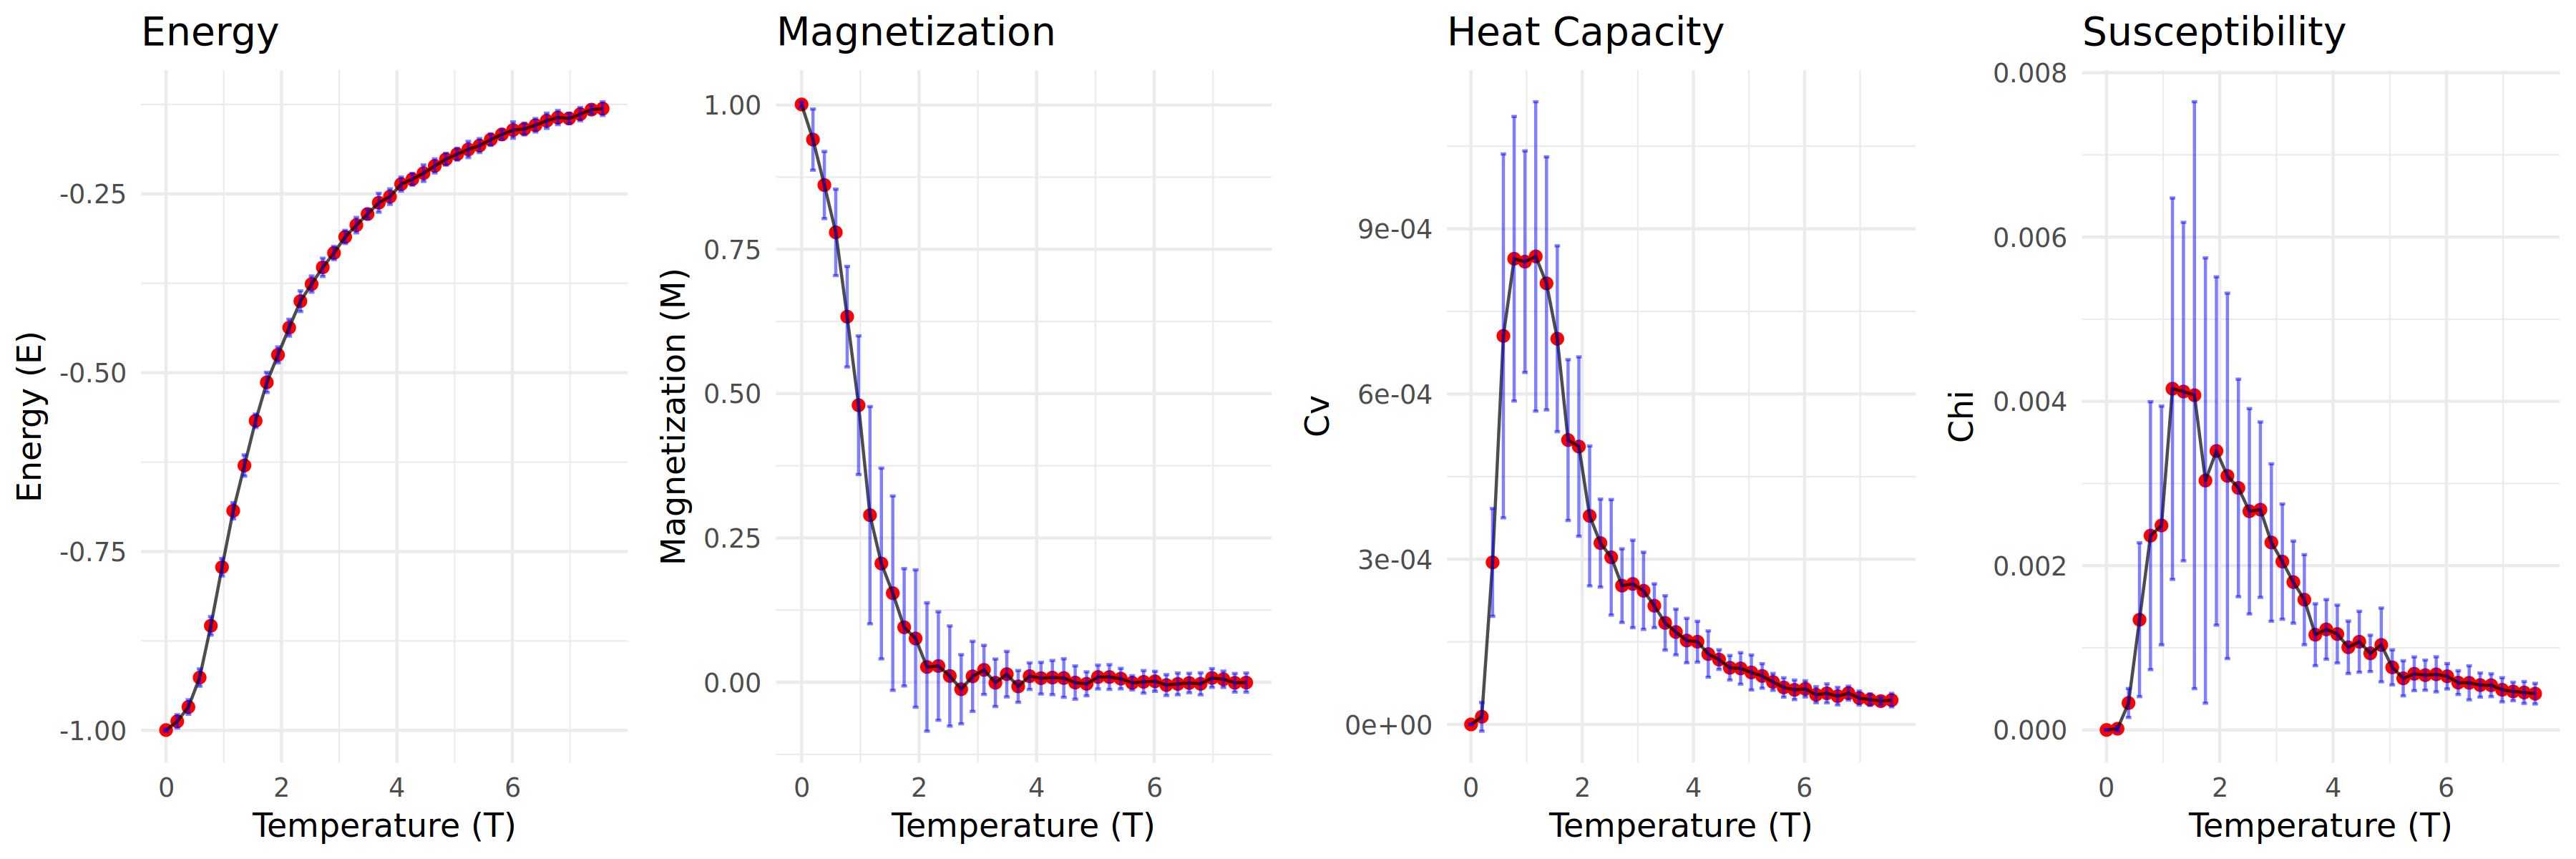
\includegraphics[width=1\linewidth]{images/IM_scale_free.png}
\end{figure}


We have got some expected results ~\cite{farside329Lectures}. As a start configuration we choose all spins up. This will traduce into an ordered phase for low temperatures (ferromagnetic). Due to the configuration choice we start from a minimal energy point and a maximum magnetization. These magnitudes will evolve as the temperature where a transition phase is made where we enter into a disordered phase (paramagnetic) where the magnetization decreases and the energy increase to 0 (approximately there will be same up and down states.

This transition is produced in the critic temperature, where the magnetization and energy change abruptly. Magnetic susceptibility and heat capacity are magnitudes that describe how the magnetization and energy change respectively, and the biggest change is produced in the critical temperature. Consequently, there will be a peak at the critic temperature. We can see that for this network, the value of the critic temperature is around T=1,0-1,5.

\textbf{Ising model for Erdos Renyi networks}

Erdos Renyi networks are simple networks to see how the Ising model behaves under different topologies. We will obtain results for different connection probabilities. This figure contains the obtained results:

\begin{figure}
    \centering
    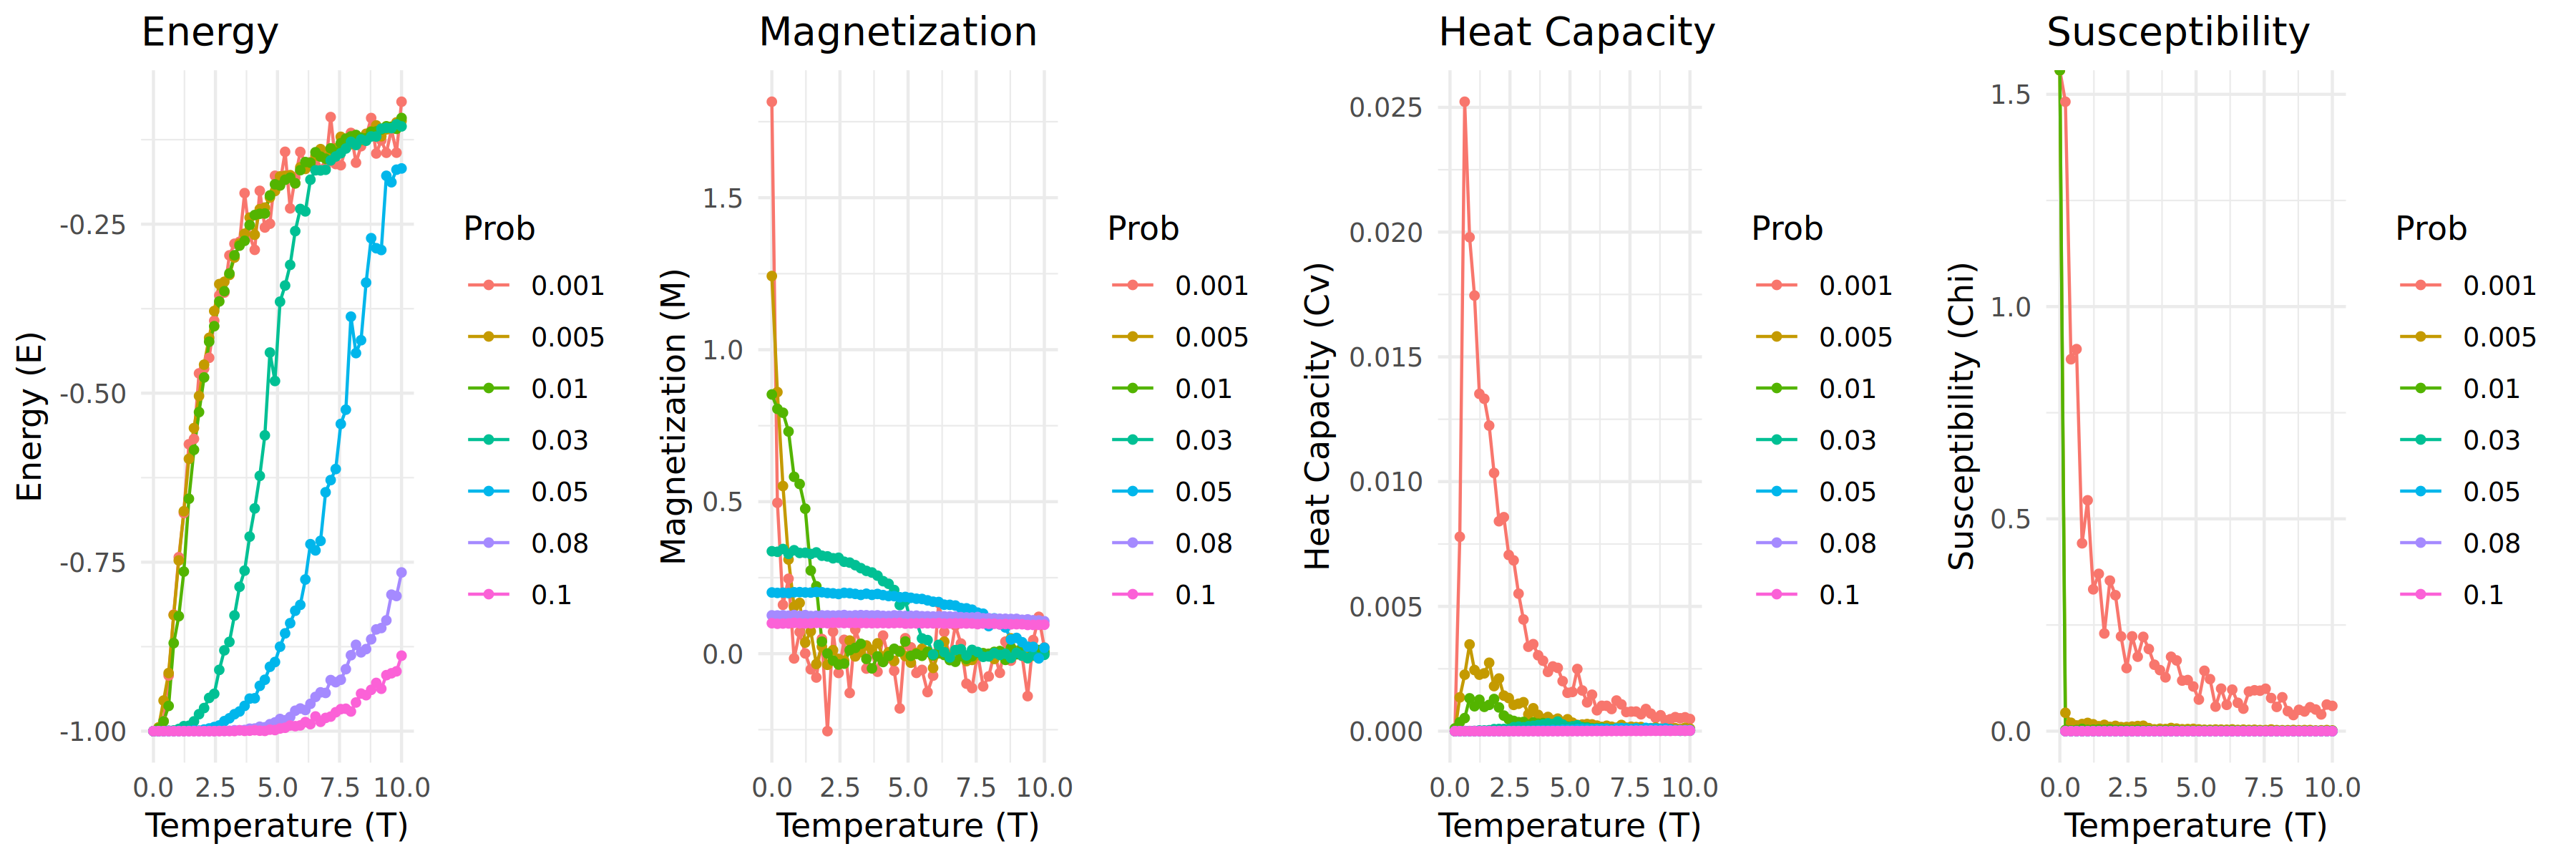
\includegraphics[width=1\linewidth, height=0.25\linewidth]{images/IM_ER.png}
\end{figure}

\newpage

As we increase the connection probability and, consequently, the mean degree of the network, the critical temperature rises. This indicates that the system requires a higher temperature to transition into the disordered phase. In the energy plot, for higher probabilities, the phase transition is pushed beyond the temperature range considered, reflecting this shift in critical temperature.

In the magnetization plot, we observe that the initial magnetization starts at lower values as the connection probability increases. This is unexpected, as magnetization should begin at 1 for T = 0.0  (corresponding to an initial all-up spin configuration). Setting this anomaly aside, we see that magnetization consistently drops to zero after passing the critical temperature, which is higher for networks with greater connectivity.

The heat capacity and susceptibility exhibit sharper peaks at lower probabilities because phase transitions occur more abruptly in less connected networks. For higher probabilities, both quantities show lower and broader peaks, indicating a smoother transition into the disordered phase.

In summary, less connected networks require a lower temperature to enter the disordered phase. This is because the Ising model dynamics propagate more easily in simpler networks with fewer connections. In contrast, more connected networks are more resistant to disorder, as each node is influenced by a larger number of neighbors, requiring higher temperatures to disrupt the ordered state.

 



\newpage